%; whizzy paragraph -pdf xpdf -latex ./whizzypdfptex.sh
%; whizzy-paragraph "^\\\\begin{frame}"
% latex beamer presentation.
% platex, latex-beamer $B$G%3%s%Q%$%k$9$k$3$H$rA[Dj!#(B 

%     Tokyo Debian Meeting resources
%     Copyright (C) 2009 Junichi Uekawa

%     This program is free software; you can redistribute it and/or modify
%     it under the terms of the GNU General Public License as published by
%     the Free Software Foundation; either version 2 of the License, or
%     (at your option) any later version.

%     This program is distributed in the hope that it will be useful,
%     but WITHOUT ANY WARRANTY; without even the implied warranty of
%     MERCHANTABILITY or FITNESS FOR A PARTICULAR PURPOSE.  See the
%     GNU General Public License for more details.

%     You should have received a copy of the GNU General Public License
%     along with this program; if not, write to the Free Software
%     Foundation, Inc., 51 Franklin St, Fifth Floor, Boston, MA  02110-1301 USA

\documentclass[cjk,dvipdfm,12pt]{beamer}
\usetheme{Tokyo}
\usepackage{monthlypresentation}

%  preview (shell-command (concat "evince " (replace-regexp-in-string "tex$" "pdf"(buffer-file-name)) "&"))
%  presentation (shell-command (concat "xpdf -fullscreen " (replace-regexp-in-string "tex$" "pdf"(buffer-file-name)) "&"))
%  presentation (shell-command (concat "evince " (replace-regexp-in-string "tex$" "pdf"(buffer-file-name)) "&"))
%  presentation (shell-command (concat "evince " (replace-regexp-in-string "tex$" "pdf"(buffer-file-name)) "&"))

%http://www.naney.org/diki/dk/hyperref.html
%$BF|K\8l(BEUC$B7O4D6-$N;~(B
\AtBeginDvi{\special{pdf:tounicode EUC-UCS2}}
%$B%7%U%H(BJIS$B7O4D6-$N;~(B
%\AtBeginDvi{\special{pdf:tounicode 90ms-RKSJ-UCS2}}

\title{$BEl5~%(%j%"(B Debian $BJY6/2q(B}
\subtitle{$B;qNA(B}
\author{$B4d>>(B $B?.MN(B iwamatsu@debian.or.jp\\IRC nick: iwamatsu}
\date{2009$BG/(B9$B7n(B16$BF|(B}
\logo{
\includegraphics[width=8cm]{image200607/openlogo-light.eps}}

%begin of commandline0
\newenvironment{commandline0}%
{\VerbatimEnvironment
  \begin{Sbox}\begin{minipage}{0.95\hsize}\begin{fontsize}{9}{9} \begin{BVerbatim}}%
{\end{BVerbatim}\end{fontsize}\end{minipage}\end{Sbox}
  \setlength{\fboxsep}{10pt}

\vspace{10pt}% skip before
\fcolorbox{dancerdarkblue}{dancerlightblue}{\TheSbox}

\vspace{6pt}% skip after
}
%end of commandline0

\begin{document}

\frame{\titlepage{}}

\emtext{$B@_1D=`Hw$K$46(NO$/$@$5$$(B}

\section{}
\begin{frame}
 \frametitle{Agenda}
\begin{minipage}[t]{0.45\hsize}
  \begin{itemize}
  \item $BCm0U;v9`(B
	\begin{itemize}
	 \item $BFC$K$J$7(B
	\end{itemize}
  \item $B:G6a$"$C$?(BDebian$B4XO"$N%$%Y%s%HJs9p(B
	\begin{itemize}
	 \item $BA02s$NJY6/2q(B
	\end{itemize}
 \end{itemize}
\end{minipage} 
\begin{minipage}[t]{0.45\hsize}
 \begin{itemize}
  \item GPG $B%-!<%5%$%s%Q!<%F%#$N@bL@(B
  \item GPG $B%-!<%5%$%s%Q!<%F%#$r3Z$K:Q$^$;$k$?$a$N%D!<%k(B caff $B$N>R2p(B
  \item $B%-!<%5%$%s%Q!<%F%#(B
 \end{itemize}
\end{minipage}
\end{frame}

\section{$B:G6a(B}

\begin{frame}
 \frametitle{2009$BG/(B8$B7n(B}
\begin{minipage}[t]{0.45\hsize}
  \begin{itemize}
  \item $BCm0U;v9`(B
	\begin{itemize}
	 \item $B0{?)6X;_(B
	\end{itemize}
  \item $B:G6a$"$C$?(BDebian$B4XO"$N%$%Y%s%HJs9p(B
	\begin{itemize}
	 \item $BA02s$NJY6/2q(B
	\end{itemize}
 \end{itemize}
\end{minipage} 
\begin{minipage}[t]{0.45\hsize}
 \begin{itemize}
  \item Debian JP Project $B2qD9="G$$N0';"(B
  \item Debconf9 $BJs9p2q(B
  \item $B2F5Y$_$N=IBj(B
 \end{itemize}
\end{minipage}
\end{frame}

\begin{frame}{Hack Cafe}

$BKh=5?eMKF|!"=5$K0l2sEl5~$N$I$C$+$N%+%U%'$G%O%C%/!#(B\\
\url{http://twitter.com/debian_hackcafe}\\
$B4X@>$G$b;O$a$?$h$&$G$9!#(B\\
($B:#F|$O(BHack Cafe$B$b7s$M$F$$$^$9!#(B)
\end{frame}

\begin{frame}{2009$BG/7W2h(B}

{\scriptsize
 \begin{enumerate}
  \item $B?7G/$N4k2h(B ($B%"%s%5%s%V%k2.7&3+:E(B)
  \item OSC Tokyo
  \item VAIO P $B%$%s%9%H!<%k5-O?!"(B
	$B%+!<%M%kFI=q2q!!%G%#%9%H%j%S%e!<%7%g%sBg=89g(B($B>.NS$5$s(B)($BEl5~Bg3X(B?)
  \item Git Handson ($B4d>>(B)($B$"$s$5$s$V$k2.7&(B?)
  \item $B2H(BDebian$B%5!<%P(B vs $B?&>l$N%M%C%H%o!<%/(B($B@iBeED6hETN)?^=q4[(B?\footnote{\url{http://www.library.chiyoda.tokyo.jp/}})
  \item DDTSS 
  \item $B%9%Z%$%s$K$F3+:E(B
  \item Debconf$BJs9p2q(B
  \item Asterisk ($BEl5~Bg3X(B?)$B!"(Budev + HAL
  \item OSC Fall?$B!!(B(10$B7n(B30$B!&(B31$BF|(B)
  \item 3D graphics $B3+H/(B 
  \item Debian $B%5!<%P(B+VMware + $B3F<o(BOS$B!"(B
	$BB>$N2>A[2=%D!<%k(B(vserver etc.)$B!"(B
	$BK:G/2q(B
 \end{enumerate}
}
\end{frame}
\emtext{GPG $B%-!<%5%$%s%Q!<%F%#$N@bL@(B}

\begin{frame}{$B$J$<%-!<%5%$%s$9$k$N$+!)(B}

\end{frame}

\begin{frame}{$B$J$<%-!<%5%$%s$9$k$N$+!)(B}
\begin{center}
\Huge $B%j%"=<(B
\end{center}
\end{frame}

\begin{frame}{$B$J$<%-!<%5%$%s$9$k$N$+!)(B}
\begin{center}
PGP/GnuPG$B$N8x3+80$r%=!<%7%c%k$J>pJs$H$H$b$K8r49$7!"?.Mj$NNX(B(web of
 trust)$B$r9-$2$k!#(B
\end{center}
\end{frame}

\begin{frame}{$B%U%j!<%=%U%H%&%'%"3+H/<T$N>l9g(B}
\begin{itemize}
\item $B<+J,$N>ZL@!J%a!<%k$K%5%$%s!?0E9f2=$7$FAw$C$?$j!#!K$KMxMQ!#(B
\item $B%=%U%H%&%'%"$N%j%j!<%9;~$K;H$C$?$j!#(B
\item Debian $B$G$O%Q%C%1!<%8$N%5%$%s!"EjI<$J$I$K;H$&!#(B
\end{itemize}
\end{frame}

\begin{frame}[containsverbatim]{$B%f!<%6$N>l9g$O!)(B}
Debian $B3+H/<T$K$J$k$?$a$NDL2a57Ni!#(B
\end{frame}

\begin{frame}[containsverbatim]{$B%f!<%6$N>l9g$O!)(B}
Linux $B%+!<%M%k$N%j%j!<%9%A%'%C%/!#$A$c$s$H(B Linus $B$,%?%0$rBG$C$F$$$k$N$+!*(B
\begin{commandline}
$ $git tag -v v2.6.31
object 74fca6a42863ffacaf7ba6f1936a9f228950f657
type commit
tag v2.6.31
tagger Linus Torvalds <torvalds@linux-foundation.org> 1252534447 -0700

Linux 2.6.31
gpg: 2009$BG/(B09$B7n(B10$BF|(B 07$B;~(B14$BJ,(B11$BIC(B JST$B$K(BDSA$B80(BID 76E21CBB$B$G;\$5$l$?=pL>(B
gpg: $B=pL>$r8!::$G$-$^$;$s(B: $B8x3+80$,8+$D$+$j$^$;$s(B
error: could not verify the tag 'v2.6.31'
\end{commandline}
\end{frame}

\begin{frame}[containsverbatim]{$B%f!<%6$N>l9g$O!)(B}
Debian $B$N>l9g$O(B secure-apt $B$G;H$o$l$F$$$k!#(B
\begin{commandline}
# apt-get update
.....
W: GPG error: http://cdn.debian.or.jp testing Release: The following
 signatures couldn't be verified because the public key is not
 available: NO_PUBKEY 9AA38DCD55BE302B
\end{commandline}
\end{frame}

\begin{frame}[containsverbatim]{$B%f!<%6$N>l9g$O!)(B}
\begin{commandline}
# gpg --keyserver wwwkeys.eu.pgp.net --recv-keys 9AA38DCD55BE302B
# gpg --armor --export 9AA38DCD55BE302B | apt-key add -
# apt-get update
.....
Fetched 2B in 1s (1B/s)
Reading package lists... Done
\end{commandline}
\Huge $B%(%i!<$,$G$J$/$J$C$?!*$3$l$GBg>fIW$G$9!*(B($B$C$F=q$$$F$"$k(BWeb$B%5%$%HB?(B
 $B$$$h$M!#(B)
\end{frame}

\begin{frame}[containsverbatim]{$B%f!<%6$N>l9g$O!)(B}
\Huge $B$8$c$J$/$F!"$A$c$s$H80$r%A%'%C%/$7$^$7$g$&!#(B
\end{frame}

\emtext{GPG $B%-!<%5%$%s%Q!<%F%#$r3Z$K:Q$^$;$k$?$a$N%D!<%k(B caff $B$N>R2p(B}

\begin{frame}{$BAj<j$K80$rAw$k$^$G$,%-!<%5%$%s%Q!<%F%#$G$9(B}
$BAj<j$K80$rAw$k$^$G$,%-!<%5%$%s%Q!<%F%#$G$9!#(B
$B$A$c$s$HAj<j$K=pL>$7$?80$rAw$j$^$7$g$&!#(B
\end{frame}

\begin{frame}{$B%-!<%5%$%s$NN.$l(B}
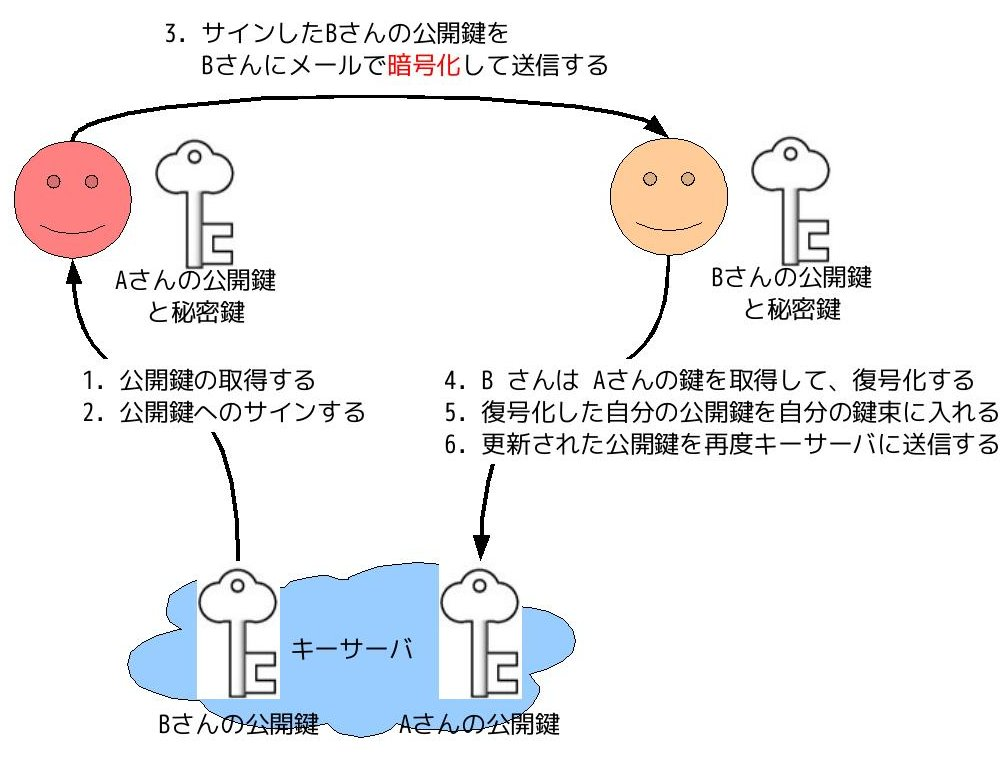
\includegraphics[width=1\hsize]{image200909/gpg-key.jpg}
\end{frame}

\begin{frame}[containsverbatim]{gpg $B$N%3%^%s%I$G$d$C$?>l9g(B}
\begin{commandline}
$ gpg --keyserver pgp.mit.edu --recv-key 40AD1FA6
$ gpg --fingerprint 40AD1FA6
$ gpg --edit-key 40AD1FA6
$ gpg --sign-key 40AD1FA6
$ gpg --check-sig 40AD1FA6                   
$ gpg --export -a 40AD1FA6 > iwamatsu.gpgkey   
$ iwamatsu.gpgkey $B$r(B $BAj<j$K%a!<%k$K(B $B=pL>(B+$B0E9f2=$7$FAw?.(B
\end{commandline}
\end{frame}

\begin{frame}
\Huge $B?t?M$J$i$$$$$1$I!"(B100$B?M$H$+$d$C$F$i$l$s!*(B
\end{frame}

\begin{frame}
\Huge $B$=$3$G(Bcaff$B$NEP>l(B
\end{frame}

\begin{frame}[containsverbatim]{$B%$%s%9%H!<%k(B}
caff $B$O(B signing-party $B%Q%C%1!<%8$GDs6!$5$l$F$$$k!#(B
\begin{commandline}
$ apt-get install signing-party
\end{commandline}
\end{frame}

\begin{frame}[containsverbatim]{$B=i4|2=(B}
caff $B$r;H$&$?$a$N=i4|2=$r9T$&!#(B
\begin{commandline} 
$ caff
.......
#
#Regards,
#{$owner}
#EOM

Please edit /home/hoge/.caffrc and run caff again.
\end{commandline}
\end{frame}

\begin{frame}[containsverbatim]{caff$B$N@_Dj(B}
\~{}/.caffrc $B$K$"$k(B $B@_Dj%U%!%$%k$r=$@5$9$k!#(B
\begin{commandline}
$ cat ~/.caffrc

$CONFIG{'owner'} = 'Nobuhiro Iwamatsu';
$CONFIG{'email'} = 'iwamatsu@debian.org';

$CONFIG{'keyid'} = [ qw{4121C7433170EBE9 32247FBB40AD1FA6} ]

# Additionally encrypt messages for these keyids
$CONFIG{'also-encrypt-to'} = [ qw{4121C7433170EBE9 32247FBB40AD1FA6} ]

# Mail template to use for the encrypted part
$CONFIG{'mail-template'} = << 'EOM'\maketitle#Hi,

please find attached the user id{(scalar @uids >= 2 ? 's' : '')}
{foreach $uid (@uids) {
    $OUT .= ``\t''.$uid.''\n'';
};}of your key {$key} signed by me.
......

\end{commandline}
\end{frame}

\begin{frame}[containsverbatim]{caff$B$N@_Dj(B}                                                                                                                                                                   
caff $B$N%G%U%)%k%H$N@_Dj$G$O!"(Bcert-digest-algo $B$,(B SHA1 $B$K$J$C$F$$$k$N$G!"(B
 \footnote{http://bugs.debian.org/cgi-bin/bugreport.cgi?bug=527944} SHA256$B$K(B
 $B@_Dj$9$k!#(B
\begin{commandline}
$ mkdir -p ~/.caff/gnupghome/
$ cat >> ~/.caff/gnupghome/gpg.conf
cert-digest-algo SHA512
personal-digest-preferences SHA512
EOF
\end{commandline}
\end{frame}

\begin{frame}[containsverbatim]{$B%m!<%+%k(BSMTP$B$N@_Dj(B}
$B%m!<%+%k!J:n6H$9$k%^%7%s!K$N(BSMTP$B$r@_Dj$7$F$*$/I,MW$,$"$k!#(B
\end{frame}

\begin{frame}[containsverbatim]{caff$B$r;H$C$?%5%$%s(B}
$B%5%$%s$9$k(BID $B$r%-!<%5!<%P$+$i<hF@$7!";XDj$7$?<+J,$N(BID$B$G%5%$%s$7$F$/$l$k!#(B
$B$=$7$F!"%5%$%s$7$?80$r0E9f2=$7$FAw?.$7$F$/$l$k!#(B

\begin{commandline}
$ caff -u $B<+J,$N(BID $B%5%$%s$9$k(BID .......                                                                                                                                                            
\end{commandline}

\end{frame}

\begin{frame}[containsverbatim]{$B%5%$%s40N;8e(B}
$B%5%$%s8e$N%G!<%?$O(B \~{}/.gnupg/pubring.gpg $B$G$O$J$/!"(B{\bf \~{}/.caff/gnupghome/pubring.gpg} $B$K3JG<(B
 $B$5$l$k!#$3$N80B+$r(B \~{}/gnupg/pubring.gpg $B$K(B $B<h$j9~$`!#(B
\begin{commandline}
$ gpg --import ~/.caff/gnupghome/pubring.gpg
\end{commandline}

$B<h$j9~$s$@$i!"<+J,$N80$r%-!<%5!<%P$KAw?.!#(B
\begin{commandline}
$ gpg --keyserver pgp.nic.ad.jp --send-keys $B<+J,$N(BID
$ gpg --keyserver pgp.mit.edu --send-keys $B<+J,$N(BID
\end{commandline}


\end{frame}


\emtext{$B%-!<%5%$%s%Q!<%F%#(B}

\begin{frame}{$B%-!<%5%$%s%Q!<%F%#(B}
\Huge $B$_$s$J$G(B sha256$B%O%C%7%e$r%A%'%C%/$7$^$7$g$&!#(B
\end{frame}

\begin{frame}{$B%-!<%5%$%s%Q!<%F%#(B}
\begin{center}
\Huge 7be4 db5f 8cef 8aa5 \\
\Huge 70d8 f3ac b564 8d7d \\
\Huge ef81 739e 6298 1b5b \\
\Huge 004a a646 44ab 00a7 \\
\end{center}

\end{frame}

\end{document}

;;; Local Variables: ***
;;; outline-regexp: "\\([ 	]*\\\\\\(documentstyle\\|documentclass\\|emtext\\|section\\|begin{frame}\\)\\*?[ 	]*[[{]\\|[]+\\)" ***
;;; End: ***
